% ======================================================================
% JECRC University -- Minor Project Report Template (LaTeX)
% Department of Computer Science and Engineering
% Session: 2025--26
% ======================================================================
\documentclass[12pt,a4paper]{report}

% ----------------------------------------------------------------------
% Packages
% ----------------------------------------------------------------------
\usepackage[a4paper,top=1in,bottom=1in,left=1.5in,right=1in]{geometry}
\usepackage{fontspec}
\setmainfont{Times New Roman}
\newfontfamily{\garamondfont}{Garamond}
\usepackage{setspace}                             % line spacing
\usepackage{graphicx}                             % figures
\usepackage{caption}                              % caption control
\usepackage{booktabs}                             % professional tables
\usepackage{array}                                % table extras
\usepackage{amsmath}                              % math helpers
\usepackage{titlesec}                             % heading formatting
\usepackage{titletoc}                             % TOC formatting
\usepackage{hyperref}                             % clickable links
\usepackage{enumitem}                             % list control
\usepackage{indentfirst}                          % indent first paragraph
\usepackage{lipsum}                               % dummy text (REMOVE for final)
\usepackage{tikz}                                 % diagrams
\usetikzlibrary{arrows.meta,positioning,shapes.geometric,calc,fit,backgrounds}
\usepackage{ragged2e}                             % better justification control

% 1.5 line spacing for body text
\onehalfspacing

% ----------------------------------------------------------------------
% Font size commands
% ----------------------------------------------------------------------
\newcommand{\chaptertitlefont}{\fontsize{18pt}{21.6pt}\selectfont\bfseries}
\newcommand{\firstorderfont}{\fontsize{16pt}{19.2pt}\selectfont\bfseries}
\newcommand{\secondorderfont}{\fontsize{14pt}{16.8pt}\selectfont\bfseries}
\newcommand{\thirdorderfont}{\fontsize{12pt}{14.4pt}\selectfont\bfseries}
\newcommand{\abstracttitlefont}{\fontsize{16pt}{19.2pt}\selectfont\bfseries\itshape}
\newcommand{\abstracttextfont}{\fontsize{12pt}{14.4pt}\selectfont\itshape}
\newcommand{\chapterrule}{\noindent\rule{\linewidth}{2.25pt}}

% Caption font: Garamond 10pt Bold Centered
\DeclareCaptionFont{mycaptionfont}{\garamondfont\fontsize{10pt}{12pt}\selectfont\bfseries}
\captionsetup{font=mycaptionfont,justification=centering}

% ----------------------------------------------------------------------
% Heading styles via titlesec
% ----------------------------------------------------------------------
% Chapter (numbered): 18pt bold, Left-aligned, thick rule below
\titleformat{\chapter}[block]
  {\raggedright\chaptertitlefont}
  {\thechapter.\hspace{0.5em}}
  {0pt}
  {}[\vspace{0.5\baselineskip}\chapterrule]
\titlespacing*{\chapter}{0pt}{0pt}{12pt}

% Chapter (unnumbered - DECLARATION, CERTIFICATE, etc.): 18pt bold, Left-aligned, thick rule below
\titleformat{name=\chapter,numberless}[block]
  {\raggedright\chaptertitlefont}
  {}
  {0pt}
  {}[\vspace{0.5\baselineskip}\chapterrule]
\titlespacing*{name=\chapter,numberless}{0pt}{12pt}{12pt}

% Section (1st order): 16pt bold, Left-aligned, 12pt before
\titleformat{\section}
  {\raggedright\firstorderfont}
  {\thesection\hspace{0.5em}}
  {0pt}
  {}
\titlespacing*{\section}{0pt}{12pt}{0pt}

% Subsection (2nd order): 14pt bold, Left-aligned, 12pt before
\titleformat{\subsection}
  {\raggedright\secondorderfont}
  {\thesubsection\hspace{0.5em}}
  {0pt}
  {}
\titlespacing*{\subsection}{0pt}{12pt}{0pt}

% Subsubsection (3rd order): 12pt bold, Left-aligned, 12pt before
\titleformat{\subsubsection}
  {\raggedright\thirdorderfont}
  {\thesubsubsection\hspace{0.5em}}
  {0pt}
  {}
\titlespacing*{\subsubsection}{0pt}{12pt}{0pt}

% ----------------------------------------------------------------------
% TOC formatting
% ----------------------------------------------------------------------
\titlecontents{chapter}
  [0pt]{\vspace{6pt}\bfseries}
  {\makebox[7em][l]{Chapter \thecontentslabel.}}
  {}
  {\hfill\contentspage}
  []

\titlecontents{section}
  [1.5em]{\vspace{2pt}}
  {\contentslabel[\thecontentslabel]{2.3em}}
  {\hspace*{-2.3em}}
  {\hfill\contentspage}
  []

\titlecontents{subsection}
  [3.8em]{\vspace{1pt}}
  {\contentslabel[\thecontentslabel]{3.2em}}
  {\hspace*{-3.2em}}
  {\hfill\contentspage}
  []

% Remove dotted leaders from TOC
\makeatletter
\renewcommand{\@dotsep}{10000}
\makeatother

% ----------------------------------------------------------------------
% Hyperref setup
% ----------------------------------------------------------------------
\hypersetup{
    colorlinks=false,
    pdfborder={0 0 0},
    pdftitle={Minor Project Report},
    pdfauthor={Student Name},
    pdfsubject={Minor Project Report -- JECRC University}
}

% ----------------------------------------------------------------------
% Custom list spacing
% ----------------------------------------------------------------------
\setlist{nosep}

% ======================================================================
% DOCUMENT BEGINS
% ======================================================================
\begin{document}
\pagestyle{plain}

% ======================================================================
% COVER PAGE
% ======================================================================
\begin{titlepage}
    \thispagestyle{empty}
    \newgeometry{top=1in,bottom=1in,left=1in,right=1in}
    \vspace*{\fill}
    \begin{center}
        {\fontsize{18pt}{22pt}\selectfont\bfseries MINOR PROJECT REPORT\par}
        \vspace{0.5cm}
        {\Large on\par}
        \vspace{0.5cm}
        {\Huge\bfseries ReportRx\par}
        \vspace{1cm}
        {\Large Submitted in partial fulfilment\par}
        \vspace{0.5cm}
        {\Large\bfseries BACHELOR OF TECHNOLOGY\par}
        {\Large\bfseries in\par}
        {\Large\bfseries COMPUTER SCIENCE AND ENGINEERING\par}

        \vspace{1.5cm}

        {\large\bfseries Submitted By:\par}
        \vspace{0.3cm}
        {\large\bfseries Gargi Mathur (Registration No. 23BCON1045)\par}
        {\large\bfseries Udit Agarwal (Registration No. 23BCON1073)\par}

        \vspace{0.5cm}
        {\large Under the Supervision of\par}
        {\large\bfseries Aneesh Mishra\par}
        {\large\bfseries Assistant Professor\par}

        \vspace{1.5cm}

        {\large\bfseries Department of Computer Science \& Engineering\par}
        {\large\bfseries Session: 2025--26\par}
        {\large\bfseries JECRC University, Jaipur\par}
    \end{center}
    \vspace*{\fill}
    \restoregeometry
\end{titlepage}

% ======================================================================
% DECLARATION (page i)
% ======================================================================
\pagenumbering{roman}
\setcounter{page}{1}
\thispagestyle{plain}

\chapter*{DECLARATION}
\addcontentsline{toc}{chapter}{DECLARATION}

\noindent We, \textbf{Gargi Mathur} (Reg. No. 23BCON1045) and \textbf{Udit Agarwal} (Reg. No. 23BCON1073), certify that the minor project work embodied in this report entitled ``\textbf{ReportRx} --- An AI-Powered Medical Report Analysis and Guidance System'' is our own bonafide work carried out by us under the supervision of \textbf{Mr. Aneesh Mishra}, Assistant Professor, Department of Computer Science \& Engineering, \textbf{JECRC University}, Jaipur. The work is original and has not been submitted earlier as a whole or in part for the award of any degree/diploma at this or any other institution/university in India or abroad.

\vspace{1.5cm}
\noindent Place: Jaipur

\vspace{2cm}
\noindent {\firstorderfont Counter Signature}

\vspace{1.5cm}
\noindent Guide: Mr. Aneesh Mishra

\noindent Designation: Assistant Professor, Department of CSE

\vspace{1.5cm}
\noindent\begin{minipage}{0.45\textwidth}
    \hrulefill \\
    Signature of Students \\[0.2cm]
    Gargi Mathur \\[0.2cm]
    (Reg. No. 23BCON1045)
\end{minipage}
\hfill
\begin{minipage}{0.45\textwidth}
    \hrulefill \\
    Udit Agarwal \\[0.2cm]
    (Reg. No. 23BCON1073)
\end{minipage}

\clearpage

% ======================================================================
% CERTIFICATE (page ii)
% ======================================================================
\setcounter{page}{2}
\thispagestyle{plain}

\chapter*{CERTIFICATE}
\addcontentsline{toc}{chapter}{CERTIFICATE}

\noindent This is to certify that the Minor Project titled ``ReportRx --- An AI-Powered Medical Report Analysis and Guidance System'' has been successfully completed by Gargi Mathur (Reg. No. 23BCON1045) and Udit Agarwal (Reg. No. 23BCON1073) under my supervision during VI Semester of B.Tech. (CSE), JECRC University, Jaipur. The work embodies original research and development effort, and meets the requirements for the award of the degree of Bachelor of Technology in Computer Science and Engineering.

\vspace{2cm}
\noindent\begin{minipage}{0.4\textwidth}
    \hrulefill \\
    (Project Guide Signature) \\[0.2cm]
    Mr. Aneesh Mishra \\[0.2cm]
    Assistant Professor, Department of CSE \\[0.2cm]
    JECRC University, Jaipur
\end{minipage}

\vspace{2cm}
\noindent\begin{minipage}{0.3\textwidth}
    \hrulefill \\
    (HOD Signature) \\[0.2cm]
    Head, Department of CSE
\end{minipage}

\vspace{2cm}
\noindent\begin{minipage}{0.3\textwidth}
    \hrulefill \\
    (Dean Signature) \\[0.2cm]
    Dean, School of Engineering
\end{minipage}

\clearpage

% ======================================================================
% ACKNOWLEDGEMENT (page iii)
% ======================================================================
\setcounter{page}{3}
\thispagestyle{plain}

\chapter*{ACKNOWLEDGEMENT}
\addcontentsline{toc}{chapter}{ACKNOWLEDGEMENT}

\noindent We would like to express our sincere gratitude to our project supervisor, Mr. Aneesh Mishra, Assistant Professor, Department of Computer Science \& Engineering, JECRC University, Jaipur, for his invaluable guidance, continuous encouragement, and constructive feedback throughout the course of this project. His expertise in the domain and consistent availability for discussion has been instrumental in shaping this work.

\noindent We extend our heartfelt thanks to the Head of Department and the Dean of the School of Engineering for providing the necessary infrastructure and academic environment that supported this project.

\noindent We are also grateful to our peers and colleagues for their thoughtful input during discussions and testing phases. Finally, we acknowledge the open-source communities behind LlamaIndex, FastAPI, Next.js, and the broader LLM ecosystem, without whose contributions this project would not have been feasible.

\vspace{2cm}
\noindent Gargi Mathur

\noindent Udit Agarwal

\clearpage

% ======================================================================
% ABSTRACT (page iv)
% ======================================================================
\setcounter{page}{4}
\thispagestyle{plain}

% Abstract heading: 16pt Bold+Italic, Left aligned (per spec)
{\abstracttitlefont ABSTRACT}
\addcontentsline{toc}{chapter}{ABSTRACT}
\vspace{24pt}  % Two blank lines (12pt each) after heading

\noindent\begin{minipage}{0.95\textwidth}
\justifying
\abstracttextfont
Medical reports often use clinical terminology that many patients cannot interpret, causing anxiety and delays in follow-up. ReportRx is an AI-powered web application that lets users upload PDF or image reports and receive clear, lay-language summaries with general health guidance. Built with a Next.js frontend and a FastAPI backend, it uses a dual-LLM architecture: a frontier model (Claude Sonnet / GPT-4) handles summarisation, while BioMedLM helps resolve clinical terms. A Retrieval-Augmented Generation (RAG) pipeline implemented with LlamaIndex grounds responses in the uploaded document and a curated medical knowledge base to improve accuracy. A rule-based guideline engine maps findings to standard public health recommendations, and ephemeral document handling helps protect privacy. The browser-based workflow requires no account creation, so patients can understand common diagnostic reports while waiting for clinical review across desktop or mobile devices. Every result includes a disclaimer advising users to consult a qualified medical professional. The project demonstrates an ethical application of RAG and multi-model LLM pipelines for accessible healthcare information.

\vspace{12pt}
\noindent\textbf{Keywords:} Medical Report Analysis, Retrieval-Augmented Generation, Large Language Models, Healthcare AI, LlamaIndex, BioMedLM, FastAPI, Next.js
\end{minipage}

\clearpage

% ======================================================================
% TABLE OF CONTENTS
% ======================================================================
\setcounter{page}{5}
\renewcommand{\contentsname}{TABLE OF CONTENTS}
\tableofcontents
\addcontentsline{toc}{chapter}{TABLE OF CONTENTS}
\clearpage

% ======================================================================
% LIST OF TABLES
% ======================================================================
\renewcommand{\listtablename}{LIST OF TABLES}
\listoftables
\addcontentsline{toc}{chapter}{LIST OF TABLES}
\clearpage

% ======================================================================
% LIST OF FIGURES
% ======================================================================
\renewcommand{\listfigurename}{LIST OF FIGURES}
\listoffigures
\addcontentsline{toc}{chapter}{LIST OF FIGURES}
\clearpage

% ======================================================================
% LIST OF ABBREVIATIONS
% ======================================================================
\chapter*{LIST OF ABBREVIATIONS}
\addcontentsline{toc}{chapter}{LIST OF ABBREVIATIONS}

\begin{table}[h]
\centering
\caption{List of Abbreviations}
\begin{tabular}{|l|l|}
    \hline
    \textbf{Abbreviation} & \textbf{Full Form} \\
    \hline
    AI & Artificial Intelligence \\
    API & Application Programming Interface \\
    CBC & Complete Blood Count \\
    DFD & Data Flow Diagram \\
    EHR & Electronic Health Record \\
    HTML & HyperText Markup Language \\
    JSON & JavaScript Object Notation \\
    LLM & Large Language Model \\
    NLP & Natural Language Processing \\
    OCR & Optical Character Recognition \\
    RAG & Retrieval-Augmented Generation \\
    REST & Representational State Transfer \\
    UI & User Interface \\
    URL & Uniform Resource Locator \\
    \hline
\end{tabular}
\end{table}

\clearpage

% ======================================================================
% Switch to Arabic page numbering from Chapter 1 onward
% ======================================================================
\pagenumbering{arabic}
\setcounter{page}{1}

% ======================================================================
% CHAPTER 1: INTRODUCTION
% ======================================================================
\chapter{Introduction}

\section{Background of the Study}
The proliferation of diagnostic testing in modern healthcare has led to an unprecedented volume of medical reports being issued to patients. Blood panels, urinalysis, lipid profiles, thyroid function tests, radiological interpretations, and pathology reports are among the most commonly issued documents. Globally, billions of diagnostic tests are conducted annually, generating an enormous corpus of clinical data directed to patients and their healthcare providers. Despite their clinical importance, these reports are predominantly written in medical and scientific language that is inaccessible to the average patient. Reference ranges, clinical flags, and abbreviations are rarely self-explanatory, and the gap between report issuance and physician consultation can span days to weeks.

This information asymmetry has measurable consequences. Studies have indicated that patients who receive abnormal results without guidance frequently experience heightened anxiety or, conversely, fail to appreciate the significance of flagged values, leading to delayed follow-up care. Both outcomes are suboptimal from a public health perspective. A 2019 study published in the Journal of General Internal Medicine found that up to 40\% of patients receiving abnormal lab results experienced significant psychological distress while awaiting physician follow-up. While patient portals and digital health records have improved report delivery, they have done little to improve report comprehension, leaving a critical gap in the patient journey.

The emergence of large language models (LLMs) and natural language processing technologies has opened new possibilities for bridging this gap. Modern LLMs, trained on vast corpora including biomedical literature, can understand complex clinical text and generate coherent, accessible explanations for lay audiences. When combined with information retrieval techniques such as Retrieval-Augmented Generation (RAG), these models can ground their outputs in specific source documents, reducing the risk of hallucination and improving factual reliability. ReportRx leverages these capabilities to provide patients with immediate, context-aware interpretations of their medical reports, empowering them with knowledge while they await professional medical consultation.

Furthermore, the rapid digitization of healthcare records in India under the Ayushman Bharat Digital Mission has accelerated the availability of electronic medical reports. Combined with widespread smartphone penetration and affordable internet access, the technological infrastructure now exists to deploy AI-powered health literacy tools at scale. ReportRx is positioned to serve this emerging digital health ecosystem by providing an accessible, web-based platform that requires no specialised hardware or software installation. The application runs entirely in the browser, making it accessible across desktop and mobile devices, and requires no user registration or personal data storage, thus aligning with both user convenience and data privacy best practices.

\section{Problem Statement}
A large proportion of patients who receive medical reports lack the background to independently interpret their results. The delay between report receipt and professional consultation creates an unserved window during which patients may experience unnecessary anxiety or make uninformed decisions about their health. Existing general-purpose conversational AI tools, while capable of discussing medical topics, are not designed to systematically parse uploaded documents, identify out-of-range values, and produce structured, grounded analyses in a safe and disclaimered manner.

The key challenges that motivate this project are:

\begin{enumerate}
    \item \textbf{Lack of Patient-Facing Interpretation Tools:} Most existing healthcare informatics tools are built for clinicians and hospital administrators, not for the patient end-user. Patient portals typically display lab results as raw numerical values with reference ranges, placing the burden of interpretation entirely on the patient.
    \item \textbf{General-Purpose AI Limitations:} While general-purpose LLMs such as ChatGPT can answer medical questions, they are not designed for structured document analysis. They lack the ability to extract tabular data from PDFs, compare numerical values against reference ranges, and produce a consistent, structured report format with appropriate disclaimers.
    \item \textbf{Accuracy and Hallucination Risks:} Medical information is a high-stakes domain where inaccuracies can have serious consequences. Any system providing medical report interpretation must ground its outputs in the source document content and employ mechanisms to minimise hallucination, a challenge that standard chatbot architectures do not adequately address.
    \item \textbf{Privacy and Trust:} Medical documents contain highly sensitive personal information. Patients need assurance that their uploaded documents are handled confidentially and not stored or misused. Any practical solution must incorporate ephemeral document handling and clear communication about data practices.
    \item \textbf{Usability for Non-Technical Users:} The target audience includes patients of varying ages, educational backgrounds, and technological literacy levels. The system must offer an intuitive interface that requires no training to use, while still delivering comprehensive, accurate, and actionable information.
\end{enumerate}

ReportRx addresses these challenges by providing an AI-powered pipeline that: (i) accepts medical report uploads in PDF or image format; (ii) extracts and structures the textual content from these heterogeneous file formats; (iii) applies a dual-LLM architecture augmented by a RAG pipeline to produce a structured, contextually grounded analysis; and (iv) maps findings to evidence-based general health guidelines while clearly delineating the boundary between informational guidance and clinical advice.

\section{Objectives of the Project}
The primary objectives of the ReportRx project are outlined below:

\begin{enumerate}
    \item To design and build a web-based application that allows users to upload medical reports in PDF or image format and receive structured, lay-language analyses in real time, without requiring any account creation or personal data submission.
    \item To implement a dual-LLM architecture that combines a frontier general-purpose language model (Claude Sonnet / GPT-4) for fluent summarisation and explanation generation with a domain-specific biomedical model (BioMedLM) for accurate clinical terminology resolution and out-of-range value detection.
    \item To develop and deploy a Retrieval-Augmented Generation pipeline using LlamaIndex, ensuring that all model outputs are grounded in the actual content of the uploaded report and supplemented by a curated medical knowledge base, thereby minimising hallucination risk.
    \item To build a rule-based general health guideline engine that systematically maps identified out-of-range clinical parameters to standardised, evidence-based public health recommendations, and to ensure this mapping is deduplicated and contextually appropriate.
    \item To implement robust document processing capabilities supporting both PDF text extraction (via PyMuPDF) and OCR-based image extraction (via Tesseract), with appropriate error handling for unsupported or malformed file types.
    \item To design a responsive, accessible frontend interface that renders the analysis output in a clear, card-based layout with colour-coded flagging of abnormal values, collapsible sections, and a visually distinct, non-dismissible professional consultation disclaimer.
    \item To ensure responsible AI deployment through ephemeral document handling (no persistent storage of uploaded files), mandatory disclaimers on every output, and clear communication about the non-clinical, informational nature of the analysis.
    \item To evaluate the system's performance through systematic testing covering unit, integration, functional, and non-functional dimensions, with particular emphasis on response time, extraction accuracy, and output consistency.
\end{enumerate}

\section{Scope of the Project}

\subsection{In-Scope Elements}
ReportRx is scoped as an academic minor project with the following in-scope elements:

\begin{enumerate}
    \item \textbf{Supported Report Types:} Complete blood count (CBC), basic metabolic panel (BMP), comprehensive metabolic panel (CMP), lipid panel, thyroid function test (TFT), and standard urinalysis. These represent the most commonly ordered outpatient tests and cover a significant majority of routine diagnostic reports encountered in clinical practice.
    \item \textbf{Input Formats:} PDF documents (both text-based and scanned), and image files in JPG and PNG formats. The system differentiates between text-based PDFs (processed via PyMuPDF) and image-based PDFs (processed via Tesseract OCR).
    \item \textbf{Analysis Output:} The system produces a structured output comprising four sections --- (i) a lay-language summary of the entire report; (ii) key observations highlighting notable findings; (iii) a colour-coded table of out-of-range values with clinical context; and (iv) evidence-based general health guidance steps.
    \item \textbf{Language:} English-language reports only.
    \item \textbf{Deployment:} Web-based application accessible via modern web browsers on desktop and mobile devices.
\end{enumerate}

\subsection{Out-of-Scope Elements}
The following elements are explicitly out of scope for the current phase:

\begin{enumerate}
    \item \textbf{Clinical Diagnosis:} The system does not provide medical diagnoses, treatment recommendations, or medication advice under any circumstances.
    \item \textbf{Hospital Integration:} Real-time integration with hospital information systems (HIS) or electronic health record (EHR) platforms is not included.
    \item \textbf{Multi-Language Support:} Reports in languages other than English are not supported in this phase.
    \item \textbf{Data Persistence:} No patient data, uploaded reports, or analysis histories are stored. The system operates on an ephemeral, per-session basis.
    \item \textbf{Longitudinal Tracking:} Comparison of results across multiple reports over time is not supported.
    \item \textbf{Specialist Reports:} Radiology reports, pathology narratives, ECG interpretations, and other narrative-heavy or image-based specialist reports are not within scope.
\end{enumerate}

\subsection{Technology Scope}
The technology stack is confined to: Next.js (React) for the frontend; FastAPI (Python) for the backend; LlamaIndex for RAG orchestration; Claude Sonnet / GPT-4 and BioMedLM for LLM inference; PyMuPDF and Tesseract for document parsing; and Tailwind CSS for styling. No proprietary frameworks, paid licences, or enterprise tools are required beyond the LLM API access fees.

% ======================================================================
% CHAPTER 2: LITERATURE REVIEW / ANALYSIS
% ======================================================================
\chapter{Literature Review / Analysis}

\section{Related Work}
Research at the intersection of natural language processing and clinical document understanding has grown substantially over the past decade. Early work focused on named entity recognition in clinical text, with systems such as cTAKES (Clinical Text Analysis and Knowledge Extraction System) demonstrating the feasibility of automated extraction of clinical concepts from unstructured reports. These rule-based and statistical systems, however, required significant domain-specific engineering and lacked the ability to generate natural, explanatory prose. Similarly, the Apache cTAKES project, developed at the Mayo Clinic, provided a robust framework for extracting clinical information from free-text electronic medical records, but remained fundamentally a structured data extraction pipeline rather than a patient-facing interpretation tool.

The advent of transformer-based models fundamentally changed the landscape. BioBERT (Lee et al., 2020) established that pre-training on biomedical corpora significantly improves performance on clinical NLP tasks including relation extraction, question answering, and entity recognition. The authors demonstrated that BioBERT, pre-trained on PubMed abstracts and PMC full-text articles, outperformed BERT by a substantial margin across all evaluated biomedical NLP benchmarks. PubMedBERT (Gu et al., 2021) extended this work by showing that domain-specific pre-training from scratch---rather than continued pre-training of a general-domain BERT---yields superior performance on biomedical tasks. BioMedLM, developed by Stanford CRFM and MosaicML, further extended this line of work to generative settings by pre-training a 2.7-billion-parameter GPT-style model on the full PubMed corpus, enabling the generation of coherent biomedical text from trained parameters alone.

The introduction of Retrieval-Augmented Generation (Lewis et al., 2020) provided a foundational framework for combining the fluency of large language models with the factual grounding of document retrieval. The RAG architecture, as originally proposed, combined a BART-based sequence-to-sequence model with a dense passage retriever (DPR), enabling the model to retrieve and condition on relevant documents during generation. Subsequent work demonstrated that RAG architectures substantially reduce hallucination rates in knowledge-intensive tasks, making them particularly well-suited for medical document analysis where factual accuracy is paramount. Variants such as REPLUG (Shi et al., 2023) enhanced this paradigm by treating the LM as a black-box and applying an iterative retrieval loop that refines the retrieved set based on the LM's own perplexity signal. Self-RAG (Asai et al., 2023) introduced self-reflection mechanisms that allow the model to decide when retrieval is needed and to critique its own generated outputs, further improving both retrieval quality and output faithfulness.

Recent systems such as Med-PaLM 2 (Singhal et al., 2023) demonstrated that a 540-billion-parameter LLM fine-tuned on medical exam questions could achieve performance approaching that of human experts on the USMLE-style benchmarks, scoring 86.5\% on the MedQA dataset. Similarly, GPT-4 demonstrated significant medical knowledge capabilities, scoring in the top 10\% of USMLE Step 2 CK examinees. However, these frontier models operate in a general question-answering paradigm and are not specifically designed for the structured, patient-facing task of parsing an uploaded diagnostic report and producing a formatted analysis with layered content (summary, observations, flagged values, guidance). Consumer-facing medical interpretation tools such as Buoy Health and Ada Health provide symptom-checking and triage guidance through interactive chatbot interfaces, but operate primarily through structured questionnaires rather than document upload and analysis. WebMD and other health information portals offer comprehensive medical encyclopaedia content but do not provide personalised report interpretation. ReportRx targets the specific, underserved application of direct diagnostic report interpretation using a grounded, multi-model pipeline architecture.

\section{Comparative Study}
The following table summarises existing tools relevant to this domain and compares their core capabilities against the proposed ReportRx system:

\begin{table}[h]
\centering
\caption{Comparative Study of Related Systems}
\begin{tabular}{|p{1.9cm}|p{1.9cm}|p{2.2cm}|p{2.4cm}|p{1.6cm}|}
    \hline
    \textbf{Tool / System} & \textbf{Approach} & \textbf{Strength} & \textbf{Limitation} & \textbf{Report Upload?} \\
    \hline
    cTAKES & Rule-based NLP & High precision on structured EHR data & No generative output; requires expert setup & No \\
    BioBERT & Pre-trained transformer & Strong clinical entity extraction & Encoder-only; cannot generate explanations & No \\
    Med-PaLM 2 & Fine-tuned frontier LLM & Near-expert medical QA performance & Proprietary; not designed for report upload & No \\
    General ChatGPT & General LLM (no RAG) & Fluent explanations & No document grounding; hallucination risk & Limited \\
    Buoy Health & Symptom-checking chatbot & Guided symptom triage & Questionnaire-based; no document analysis & No \\
    Ada Health & AI-powered symptom assessment & Personalised health insights & No structured report parsing & No \\
    WebMD / Healthline & Encyclopaedic content & Comprehensive health reference & Generic content; not personalised to user's report & No \\
    ReportRx (Proposed) & Dual-LLM + RAG (LlamaIndex) & Grounded, structured, disclaimered output & Academic scope; English only & Yes \\
    \hline
\end{tabular}
\end{table}

The comparative analysis reveals that ReportRx occupies a unique position in the landscape: it is the only system in the comparison that combines structured document upload and parsing with AI-powered analysis, RAG-based grounding to minimise hallucination, and a privacy-preserving ephemeral processing model. While general-purpose LLMs offer conversational medical knowledge, they lack the document-centric architecture required for systematic report analysis. Conversely, dedicated medical tools such as Buoy and Ada focus on symptom assessment rather than diagnostic report interpretation.

\section{Feasibility Study}

\subsection{Technical Feasibility}
ReportRx is built entirely on well-documented, widely adopted technologies, each of which has been proven in production at scale. Next.js (version 14) provides a production-grade React framework with server-side rendering, static site generation, and API route capabilities. Its mature ecosystem supports responsive design, component-based development, and seamless deployment to Vercel's edge network. FastAPI is a high-performance Python web framework leveraging asynchronous IO (ASGI) and Pydantic-based data validation, making it suitable for building concurrent REST APIs that can handle multiple simultaneous report analysis requests without blocking. LlamaIndex offers a mature RAG orchestration layer with built-in support for over 40 document loaders, multiple vector store backends (Chroma, Pinecone, Weaviate), and flexible query engine configurations. LLM access is mediated through the Anthropic and OpenAI APIs, both of which provide stable, versioned interfaces with generous rate limits suitable for academic development. All core components are either open-source or accessible via pay-as-you-go API pricing, confirming technical feasibility within an academic setting.

One potential technical risk is the dependency on external LLM API availability. If either the Anthropic or OpenAI API experiences downtime, the system's core analysis pipeline would be unavailable. This risk is partially mitigated by the dual-LLM architecture, which provides two independent LLM backends. Additionally, the use of LlamaIndex's modular design allows the LLM provider to be swapped with minimal code changes, supporting future migration to locally hosted models if required.

\subsection{Economic Feasibility}
As an academic project, core development uses free and open-source tools exclusively. The technology stack --- Next.js, FastAPI, LlamaIndex, PyMuPDF, Tesseract --- carries no licensing costs. LLM API usage during development and testing is cost-manageable; at typical academic usage volumes (approximately 200--400 analyses per month for development and testing), monthly API costs are expected to remain under Rs.\,1,500 ($\sim$\$18 USD). The Next.js frontend can be hosted on Vercel at no cost under its free tier (100 GB bandwidth, 100 hours of serverless function execution per month), and the FastAPI backend can run on a free-tier cloud instance (e.g., Render or Railway) during the project period. No proprietary software licences, hardware purchases, or specialised infrastructure expenditures are required.

If the system were to be scaled beyond academic use, the primary cost driver would be LLM API usage. At production scale (thousands of analyses per month), optimisations such as prompt caching, response caching for similar report patterns, and model distillation could reduce per-query costs by an estimated 40--60\%. Local hosting of a quantised BioMedLM variant could further eliminate the biomedical model API cost without compromising clinical accuracy.

\subsection{Operational Feasibility}
The application interface is designed to require no prior technical knowledge from end users. The single primary interaction --- a drag-and-drop or click-to-upload file field --- is a universally understood web interaction pattern. The structured output format --- covering summary, key observations, out-of-range values, and guidance steps --- is intuitive and self-explanatory. The colour-coded flagging system (red for high values, blue for low values) provides immediate visual comprehension of abnormal results. The mandatory disclaimer at the end of every analysis, rendered in a visually distinct box with a contrasting background, ensures users understand the non-clinical nature of the output.

The system is operationally feasible for the intended audience of non-technical patients for several additional reasons: (i) no account creation or login is required, eliminating a common barrier to adoption; (ii) the application is fully responsive and functions on smartphones, which are the primary internet access device for many target users in the Indian context; (iii) the analysis completes within 30--45 seconds, a duration that is acceptable for a single document analysis task; and (iv) the output can be printed, saved as PDF, or shared directly from the browser using native sharing APIs, enabling users to share the analysis with their healthcare provider.

% ======================================================================
% CHAPTER 3: SYSTEM DESIGN
% ======================================================================
\chapter{System Design}

\section{System Architecture}
ReportRx adopts a three-tier architecture comprising a client-side frontend presentation layer, a server-side backend API layer, and an AI inference layer. This separation of concerns ensures modularity, maintainability, and the ability to independently scale or replace each tier without affecting the others.

\paragraph{Frontend Tier (Presentation Layer)}
The frontend is implemented in Next.js 14 (React) with Tailwind CSS and is responsible for file upload, request submission, loading state management, and structured result rendering. The user interface is organised into a single-page application (SPA) paradigm with client-side routing. Key UI components include: a drag-and-drop file upload zone with format validation feedback; a processing progress indicator showing the current stage of analysis (upload, extraction, analysis, guidance); and a structured output display card with five collapsible sections (Report Summary, Key Observations, Out-of-Range Values Table, General Guidance Steps, and Disclaimer). The frontend communicates with the backend exclusively through a single REST API endpoint using the Fetch API. Error states (network failure, invalid file type, server error) are handled with user-friendly error banners and retry prompts.

\paragraph{Backend Tier (API Layer)}
The backend is a FastAPI application that exposes a single primary endpoint (\texttt{POST /api/v1/analyse}) which orchestrates the complete analysis workflow. The endpoint accepts a multipart form upload containing the file and optional metadata (report type hint). The request lifecycle within the backend proceeds as follows:

\begin{enumerate}
    \item \textbf{Validation:} File type is checked against an allowed list (application/pdf, image/jpeg, image/png). File size is checked against a configurable maximum (default: 20 MB). Malformed requests are rejected with HTTP 422 and a descriptive JSON error body.
    \item \textbf{Routing:} Valid files are routed to the appropriate extraction pipeline based on MIME type --- PyMuPDF for PDF documents, Tesseract OCR for image files.
    \item \textbf{Extraction:} Text content is extracted and normalised into a plain-text string. Structural cues (table boundaries, section headers, numerical columns) are preserved where possible.
    \item \textbf{RAG Indexing:} Extracted text is chunked and embedded using the configured embedding model. Chunks are stored in an in-memory LlamaIndex VectorStoreIndex.
    \item \textbf{Retrieval:} A structured query is constructed and executed against the index, retrieving the top-k most relevant document chunks.
    \item \textbf{Inference:} Retrieved context is passed sequentially to the BioMedLM model and then to the frontier LLM (Claude Sonnet or GPT-4), producing a merged structured JSON output.
    \item \textbf{Guideline:} The guideline engine maps flagged parameters to health guidance rules and appends them to the output payload.
    \item \textbf{Response:} The final structured JSON response is serialised, returned to the frontend with HTTP 200, and the in-memory index is destroyed.
\end{enumerate}

\paragraph{AI Inference Layer}
The AI inference layer consists of external API calls to the Anthropic (Claude Sonnet) or OpenAI (GPT-4) endpoint for the frontier model, and a locally hosted or API-accessible BioMedLM instance for the biomedical model. Both models are accessed via REST API calls with structured prompt templates. The BioMedLM prompt is designed for structured parameter extraction and clinical annotation, while the frontier model prompt is designed for lay-language explanation and guidance generation. The outputs are merged by the backend orchestration logic, which reconciles the JSON schemas of both model responses and validates the final structure before passing it to the guideline engine.

% Figure: caption BELOW the figure, centered
\begin{figure}[h]
    \centering
    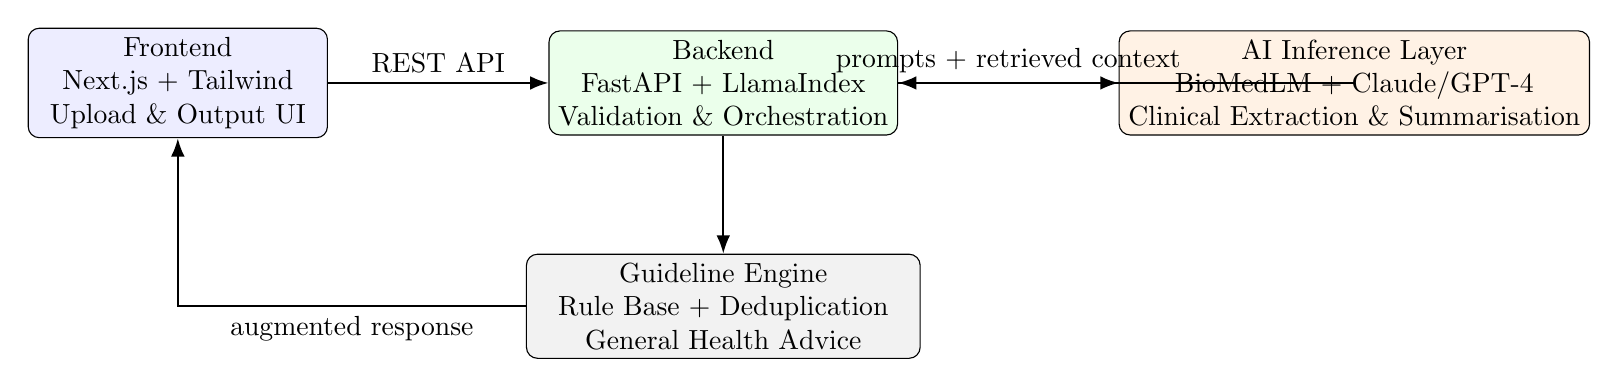
\begin{tikzpicture}[>=Latex, node distance=1.8cm]
        \tikzset{block/.style={rectangle, draw, rounded corners, align=center, minimum height=1.2cm, minimum width=3.8cm, fill=blue!7}}
        \node[block] (frontend) {Frontend\\Next.js + Tailwind\\Upload \& Output UI};
        \node[block, right=2.8cm of frontend, fill=green!8] (backend) {Backend\\FastAPI + LlamaIndex\\Validation \& Orchestration};
        \node[block, right=2.8cm of backend, fill=orange!10] (ai) {AI Inference Layer\\BioMedLM + Claude/GPT-4\\Clinical Extraction \& Summarisation};
        \node[block, below=1.5cm of backend, minimum width=5.0cm, fill=gray!10] (guide) {Guideline Engine\\Rule Base + Deduplication\\General Health Advice};
        \draw[->, thick] (frontend) -- node[above]{REST API} (backend);
        \draw[->, thick] (backend) -- node[above]{prompts + retrieved context} (ai);
        \draw[->, thick] (ai) |- (backend);
        \draw[->, thick] (backend) -- (guide);
        \draw[->, thick] (guide.west) -| node[pos=0.25, below]{augmented response} (frontend.south);
    \end{tikzpicture}
    \caption{System Architecture Diagram}
\end{figure}

\section{UML Diagrams}
Unified Modeling Language (UML) diagrams are used to visualise the system's structure and behaviour from different perspectives. Three UML diagram types are presented: a Use Case Diagram to capture functional requirements from the user's perspective, an Activity Diagram to illustrate the end-to-end processing workflow, and a Sequence Diagram to detail the interaction sequence between system components during a typical analysis session.

\subsection{Use Case Diagram}
The primary actor is the User (Patient), who interacts with the system to obtain a medical report analysis. The system use cases are:

\begin{enumerate}
    \item \textbf{Upload Medical Report:} The user selects and submits a medical report file (PDF or image) via the web interface. The system validates the file format and size before accepting it.
    \item \textbf{View Report Summary:} After processing, the system displays a concise lay-language summary of the uploaded report's contents.
    \item \textbf{View Key Observations:} The system highlights the most clinically significant findings from the report, presented in plain English.
    \item \textbf{View Out-of-Range Values:} Parameters whose measured values fall outside the stated reference range are displayed in a colour-coded table with clinical context.
    \item \textbf{View General Health Guidance:} Evidence-based lifestyle and follow-up recommendations are presented for flagged parameters.
    \item \textbf{View Professional Consultation Disclaimer:} A mandatory, non-dismissible disclaimer is displayed with every analysis, directing users to consult a qualified healthcare professional.
\end{enumerate}

A secondary actor, the AI Backend (LLM APIs), interacts with the system through API calls mediated by the FastAPI backend. The AI Backend is not directly visible to the user but is essential for the analysis pipeline.

\begin{figure}[h]
    \centering
    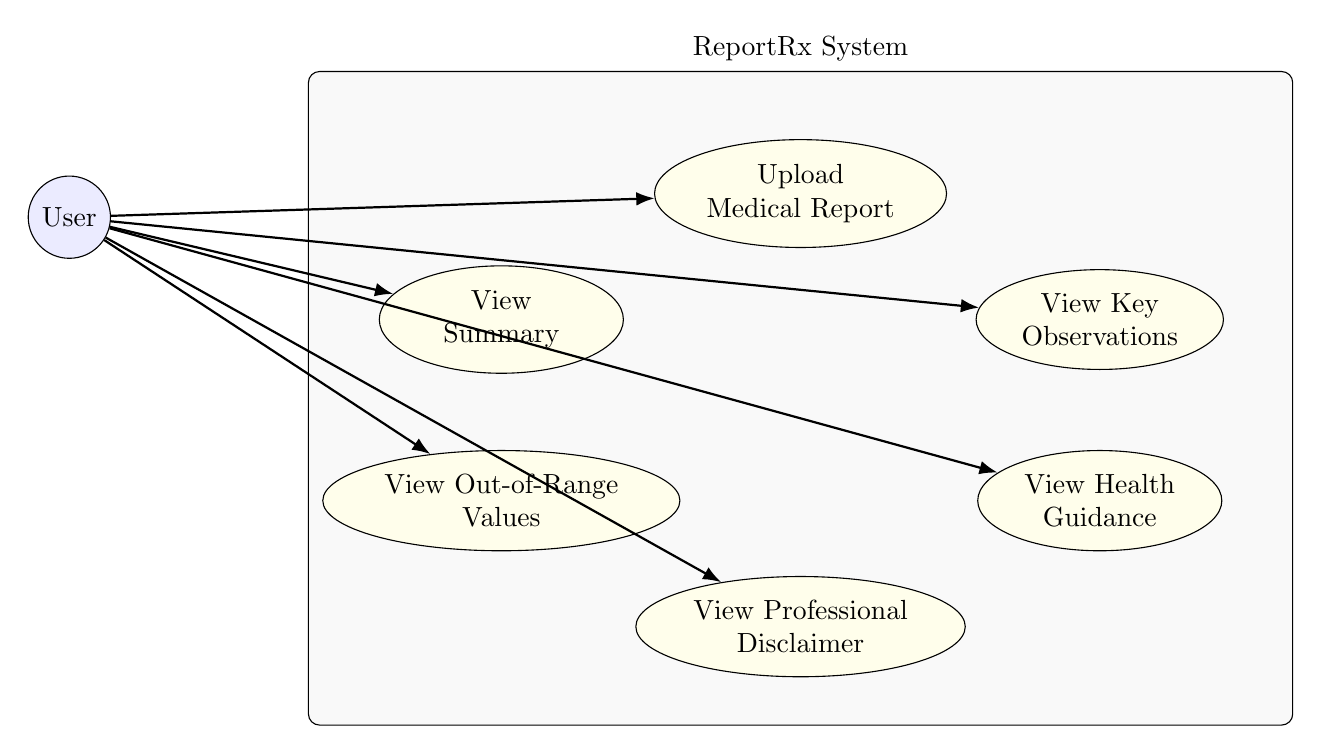
\begin{tikzpicture}[>=Latex, node distance=0.9cm]
        \tikzset{usecase/.style={ellipse, draw, align=center, minimum width=3.1cm, minimum height=0.9cm, fill=yellow!8}}
        \node[draw, rounded corners, fill=gray!5, minimum width=12.5cm, minimum height=8.3cm, label=above:{ReportRx System}] (sys) {};
        \node[draw, circle, fill=blue!8, left=2.5cm of sys.west, yshift=2.3cm] (user) {User};
        \node[usecase] (u1) at ($(sys.center)+(0,2.6)$) {Upload\\Medical Report};
        \node[usecase] (u2) at ($(sys.center)+(-3.8,1.0)$) {View\\Summary};
        \node[usecase] (u3) at ($(sys.center)+(3.8,1.0)$) {View Key\\Observations};
        \node[usecase] (u4) at ($(sys.center)+(-3.8,-1.3)$) {View Out-of-Range\\Values};
        \node[usecase] (u5) at ($(sys.center)+(3.8,-1.3)$) {View Health\\Guidance};
        \node[usecase] (u6) at ($(sys.center)+(0,-2.9)$) {View Professional\\Disclaimer};
        \draw[->, thick] (user) -- (u1);
        \draw[->, thick] (user) -- (u2);
        \draw[->, thick] (user) -- (u3);
        \draw[->, thick] (user) -- (u4);
        \draw[->, thick] (user) -- (u5);
        \draw[->, thick] (user) -- (u6);
    \end{tikzpicture}
    \caption{Use Case Diagram}
\end{figure}

\subsection{Activity Diagram}
The activity diagram models the sequential workflow of the entire analysis process from user initiation to output display. The activity flow begins with the user selecting and uploading a file. The system validates the file type and size against configured limits. On successful validation, text extraction commences via the appropriate pipeline (PyMuPDF for PDF, Tesseract OCR for images). On validation failure, an appropriate error message is returned and the user is prompted to retry. Extracted text is indexed into the LlamaIndex in-memory vector store and queried using the structured retrieval prompt. The retrieved context is passed to the dual-LLM pipeline: first to BioMedLM for clinical parameter extraction and annotation, then to the frontier LLM for lay-language summarisation. The guideline engine maps flagged parameters to health guidance rules and appends the results. The structured output is rendered in the frontend interface. At any stage, if an error occurs (extraction failure, API timeout, invalid response format), the pipeline is aborted and a descriptive error message is displayed to the user.

\begin{figure}[h]
    \centering
    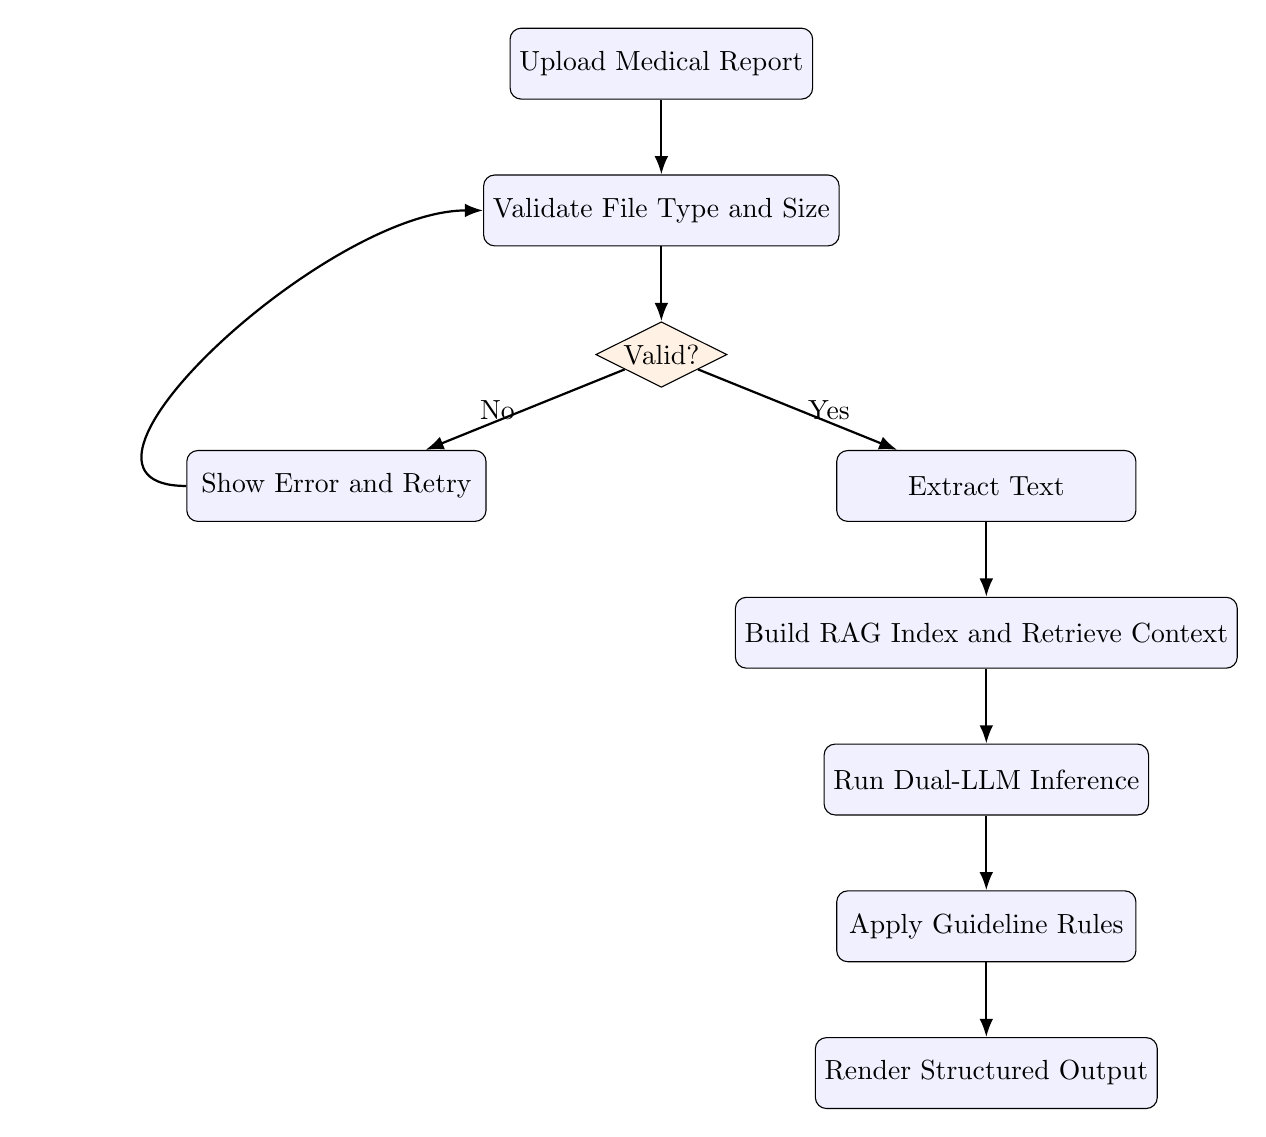
\begin{tikzpicture}[>=Latex, node distance=0.95cm]
        \tikzset{flowstep/.style={rectangle, draw, rounded corners, align=center, minimum width=3.8cm, minimum height=0.9cm, fill=blue!6}, decision/.style={diamond, draw, align=center, aspect=2, inner sep=1pt, fill=orange!10}}
        \node[flowstep] (s1) {Upload Medical Report};
        \node[flowstep, below=of s1] (s2) {Validate File Type and Size};
        \node[decision, below=of s2] (d1) {Valid?};
        \node[flowstep, below left=1.0cm and 1.8cm of d1] (s3) {Show Error and Retry};
        \node[flowstep, below right=1.0cm and 1.8cm of d1] (s4) {Extract Text};
        \node[flowstep, below=of s4] (s5) {Build RAG Index and Retrieve Context};
        \node[flowstep, below=of s5] (s6) {Run Dual-LLM Inference};
        \node[flowstep, below=of s6] (s7) {Apply Guideline Rules};
        \node[flowstep, below=of s7] (s8) {Render Structured Output};
        \draw[->, thick] (s1) -- (s2);
        \draw[->, thick] (s2) -- (d1);
        \draw[->, thick] (d1) -- node[left]{No} (s3);
        \draw[->, thick] (d1) -- node[right]{Yes} (s4);
        \draw[->, thick] (s4) -- (s5);
        \draw[->, thick] (s5) -- (s6);
        \draw[->, thick] (s6) -- (s7);
        \draw[->, thick] (s7) -- (s8);
        \draw[->, thick] (s3.west) .. controls +(-2.0,0) and +(-2.0,0) .. (s2.west);
    \end{tikzpicture}
    \caption{Activity Diagram}
\end{figure}

\subsection{Sequence Diagram}
The sequence diagram illustrates the time-ordered interaction between all system components during a typical analysis request. The key actors and components involved are: the User, the Next.js Frontend, the FastAPI Backend, the LlamaIndex RAG Engine, the Frontier LLM API (Claude Sonnet / GPT-4), the BioMedLM API, and the Guideline Engine.

The interaction sequence proceeds as follows:

\begin{enumerate}
    \item \textbf{File Upload:} The User submits a file through the Frontend. The Frontend sends a POST request to the Backend's \texttt{/api/v1/analyse} endpoint.
    \item \textbf{Validation and Extraction:} The Backend validates the file and routes it to the appropriate text extraction pipeline. Extracted text is returned to the main orchestrator.
    \item \textbf{Indexing and Retrieval:} The Backend sends the extracted text to the LlamaIndex RAG Engine for chunking, embedding, and indexing. A structured query is executed, and the top-k relevant chunks are returned.
    \item \textbf{First LLM Call (BioMedLM):} The Backend sends the retrieved context to the BioMedLM API with a structured extraction prompt. BioMedLM returns a JSON object containing identified parameters, values, reference ranges, and clinical annotations.
    \item \textbf{Second LLM Call (Frontier Model):} The Backend sends the BioMedLM outputs alongside the original context to the Frontier LLM API with a lay-language summarisation prompt. The Frontier LLM returns a JSON object containing the summary, key observations, and recommendations.
    \item \textbf{Guideline Mapping:} The Backend passes the merged LLM output to the Guideline Engine. The engine performs rule-based mapping and returns augmented output with guidance steps.
    \item \textbf{Response:} The Backend serialises the final structured response and returns it to the Frontend, which renders it for the User. The in-memory index is then destroyed.
\end{enumerate}

All LLM API calls are performed asynchronously over HTTPS, with timeouts configured at 30 seconds per call. The BioMedLM call is executed before the Frontier LLM call because the latter's prompt depends on the structured parameter output from the former.

\begin{figure}[h]
    \centering
    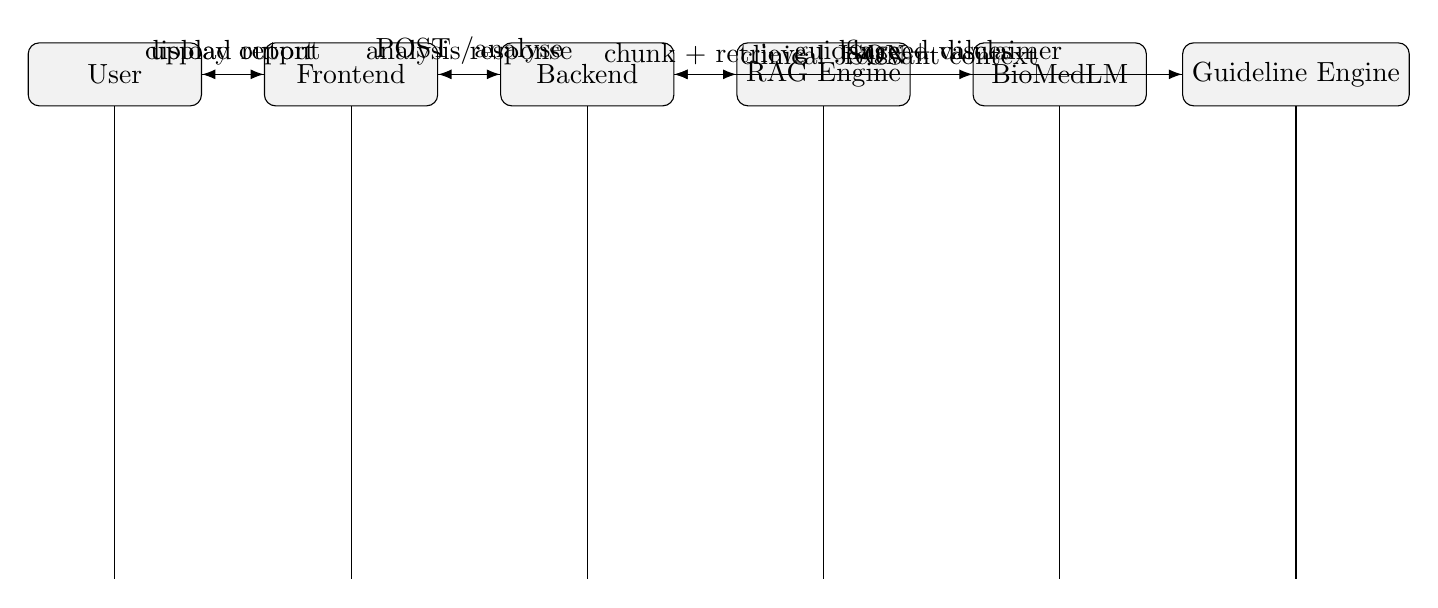
\begin{tikzpicture}[>=Latex, node distance=1.5cm]
        \tikzset{lifeline/.style={draw, thin}, actor/.style={rectangle, draw, rounded corners, fill=gray!10, minimum width=2.2cm, minimum height=0.8cm, align=center}}
        \node[actor] (u) at (0,0) {User};
        \node[actor] (f) at (3.0,0) {Frontend};
        \node[actor] (b) at (6.0,0) {Backend};
        \node[actor] (r) at (9.0,0) {RAG Engine};
        \node[actor] (m) at (12.0,0) {BioMedLM};
        \node[actor] (g) at (15.0,0) {Guideline Engine};
        \foreach \x in {u,f,b,r,m,g} {\draw[lifeline] (\x.south) -- ++(0,-6.0);}
        \draw[->] (u) -- node[above]{upload report} (f);
        \draw[->] (f) -- node[above]{POST /analyse} (b);
        \draw[->] (b) -- node[above]{chunk + retrieve} (r);
        \draw[->] (r) -- node[above]{relevant context} (m);
        \draw[->] (m) -- node[above]{clinical JSON} (b);
        \draw[->] (b) -- node[above]{flagged values} (g);
        \draw[->] (g) -- node[above]{guidance + disclaimer} (b);
        \draw[->] (b) -- node[above]{analysis response} (f);
        \draw[->] (f) -- node[above]{display output} (u);
    \end{tikzpicture}
    \caption{Sequence Diagram}
\end{figure}

\section{Data Flow Diagram (DFD)}
The Data Flow Diagram provides a structured analysis of how data moves through the system. Two levels of DFD are presented.

\paragraph{Level-0 DFD (Context Diagram)}
The Level-0 DFD depicts the entire ReportRx system as a single process --- the ReportRx Analysis Engine. The primary external entity is the User, who provides a Medical Report (PDF or Image) as input and receives a Structured Analysis Report as output. A secondary external entity is the LLM API Provider (Anthropic / OpenAI), which provides inference services. The single process encapsulates all internal operations: document ingestion, text extraction, RAG indexing and retrieval, dual-LLM inference, guideline mapping, and output formatting.

\paragraph{Level-1 DFD}
The Level-1 DFD decomposes the ReportRx Analysis Engine into four distinct sub-processes:

\begin{enumerate}
    \item \textbf{Process 1 --- Document Ingestion and Text Extraction (P1):} Accepts the raw uploaded file, validates its format and size, and extracts plain text using the appropriate parser. Outputs: Normalised text string. Data stores: None (ephemeral).
    \item \textbf{Process 2 --- RAG Indexing and Retrieval (P2):} Accepts the extracted text, splits it into overlapping chunks, generates embeddings, and stores them in an in-memory vector index. Executes a structured retrieval query and returns the most relevant chunks. Data stores: In-Memory Vector Index.
    \item \textbf{Process 3 --- Dual-LLM Inference (P3):} Accepts retrieved document chunks, invokes BioMedLM for clinical parameter extraction and the frontier LLM for summarisation, and merges the results into a structured JSON. Data stores: None.
    \item \textbf{Process 4 --- Guideline Engine and Output Formatting (P4):} Accepts the merged LLM output, performs rule-based mapping against the guideline rule base, deduplicates guidance items, appends the disclaimer, and formats the final structured response. Data stores: Guideline Rule Base (JSON).
\end{enumerate}

Data stores in the Level-1 DFD include the In-Memory Vector Index (ephemeral, destroyed after each analysis) and the Guideline Rule Base (persistent JSON configuration file).

\begin{figure}[h]
    \centering
    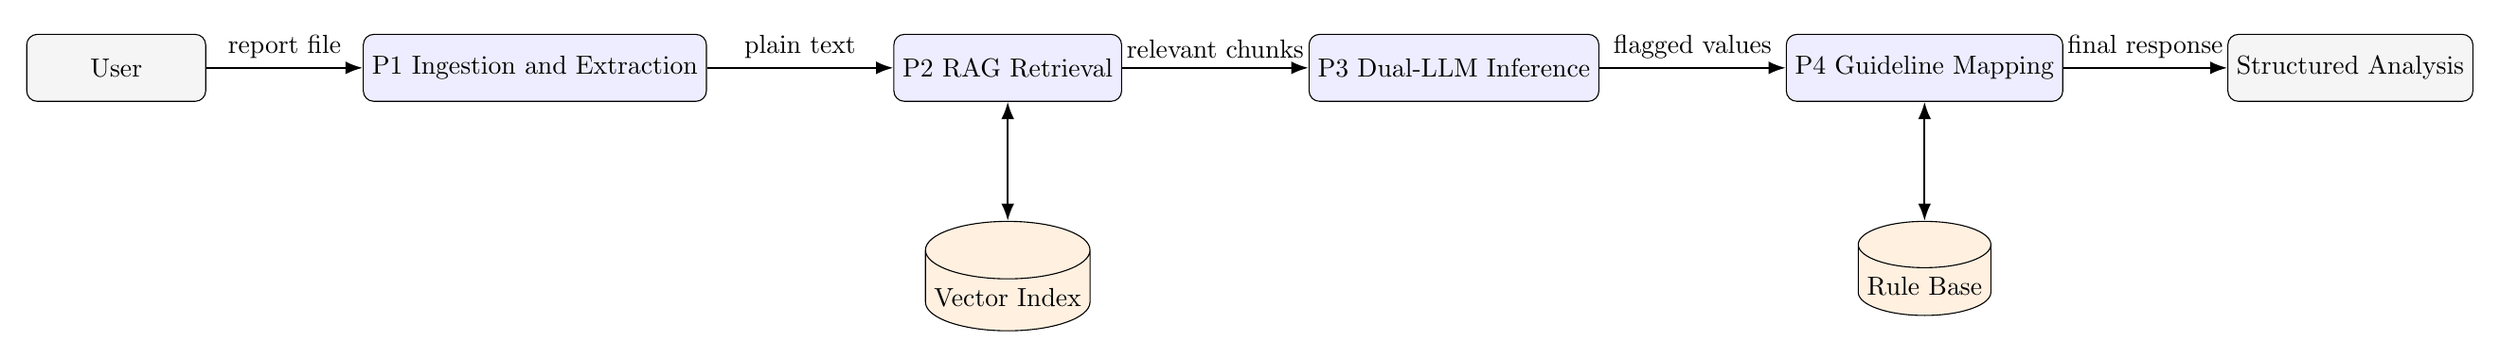
\begin{tikzpicture}[>=Latex, node distance=1.4cm]
        \tikzset{proc/.style={rectangle, draw, rounded corners, align=center, minimum width=2.9cm, minimum height=0.9cm, fill=blue!7}, store/.style={cylinder, shape border rotate=90, draw, minimum width=1.7cm, minimum height=1.1cm, aspect=0.35, fill=orange!12}, entity/.style={rectangle, draw, rounded corners, align=center, minimum width=2.4cm, minimum height=0.9cm, fill=gray!8}}
        \node[entity] (user) {User};
        \node[proc, right=2.1cm of user] (p1) {P1 Ingestion and Extraction};
        \node[proc, right=2.5cm of p1] (p2) {P2 RAG Retrieval};
        \node[proc, right=2.5cm of p2] (p3) {P3 Dual-LLM Inference};
        \node[proc, right=2.5cm of p3] (p4) {P4 Guideline Mapping};
        \node[entity, right=2.2cm of p4] (out) {Structured Analysis};
        \node[store, below=1.6cm of p2] (ds1) {Vector Index};
        \node[store, below=1.6cm of p4] (ds2) {Rule Base};
        \draw[->, thick] (user) -- node[above]{report file} (p1);
        \draw[->, thick] (p1) -- node[above]{plain text} (p2);
        \draw[->, thick] (p2) -- node[above]{relevant chunks} (p3);
        \draw[->, thick] (p3) -- node[above]{flagged values} (p4);
        \draw[->, thick] (p4) -- node[above]{final response} (out);
        \draw[<->, thick] (p2) -- (ds1);
        \draw[<->, thick] (p4) -- (ds2);
    \end{tikzpicture}
    \caption{Data Flow Diagram}
\end{figure}

\section{ER Diagram}
The Entity-Relationship (ER) diagram for ReportRx models the key data abstractions that underpin the system's document processing pipeline. Since the application follows a stateless, privacy-preserving design philosophy --- no patient data is persisted beyond the lifetime of a single analysis session --- the ER model is intentionally lean and focused on the logical flow rather than persistent storage schemas.

The primary entities and their attributes are:

\begin{itemize}
    \item \textbf{User}: Represents the individual who submits a medical report for analysis. Key attributes include a session identifier and request timestamp. No user account or personal identifiable information is stored.
    \item \textbf{Medical Report}: Represents the uploaded document. Attributes include a unique request identifier, file type (PDF or image), upload timestamp, extracted plain-text content, and processing status.
    \item \textbf{Analysis Result}: The structured output generated after processing. Attributes include analysis ID, a lay-language summary, a list of key observations, flagged out-of-range parameters (with name, value, reference range, direction, and clinical note), general health guidance steps, and the mandatory professional consultation disclaimer.
    \item \textbf{Guideline Rule}: A reference entity representing entries in the rule base. Attributes include rule ID, clinical parameter name, threshold direction (high/low), severity level, and one or more standard guidance text strings.
\end{itemize}

The relationships are straightforward: a single User submission triggers the creation of one Medical Report record; each Medical Report is processed to produce exactly one Analysis Result; and the Analysis Result references zero or more Guideline Rules to assemble the final guidance output. There is no direct relationship between different users' sessions, and no historical aggregation is performed.

\begin{figure}[h]
    \centering
    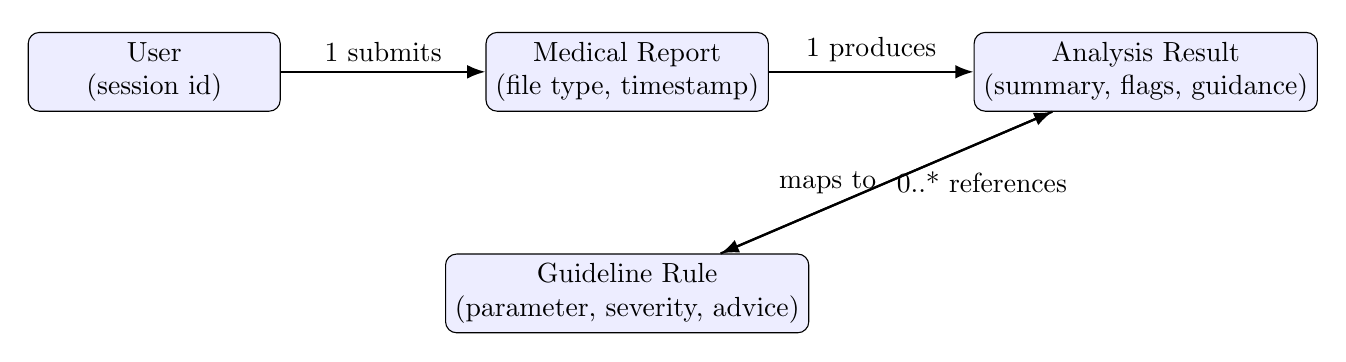
\begin{tikzpicture}[>=Latex, node distance=1.4cm]
        \tikzset{entity/.style={rectangle, draw, rounded corners, align=center, minimum width=3.2cm, minimum height=1cm, fill=blue!7}}
        \node[entity] (user) {User\\(session id)};
        \node[entity, right=2.6cm of user] (report) {Medical Report\\(file type, timestamp)};
        \node[entity, right=2.6cm of report] (result) {Analysis Result\\(summary, flags, guidance)};
        \node[entity, below=1.8cm of report] (rule) {Guideline Rule\\(parameter, severity, advice)};
        \draw[-Latex, thick] (user) -- node[above]{1 submits} (report);
        \draw[-Latex, thick] (report) -- node[above]{1 produces} (result);
        \draw[-Latex, thick] (result) -- node[right]{0..* references} (rule);
        \draw[-Latex, thick] (rule) -- node[left]{maps to} (result);
    \end{tikzpicture}
    \caption{Entity-Relationship Diagram}
\end{figure}

\section{Database Design}
ReportRx does not employ a persistent relational database for user data or uploaded documents, in accordance with the core privacy requirement that documents not be stored permanently. The only persistent data store is the Guideline Rule Base, a structured JSON configuration file that maps clinical parameter names and out-of-range conditions to standardised general health guidance text. The schema of this rule base is as follows:

\begin{verbatim}
{
  "rules": [
    {
      "parameter": "Hemoglobin",
      "condition": "low",
      "severity": "moderate",
      "guidance": [
        "Iron-rich diet (leafy greens, legumes, red meat)",
        "Consider vitamin B12 supplementation after consulting physician",
        "Schedule follow-up Complete Blood Count in 4-6 weeks"
      ]
    },
    ...
  ]
}
\end{verbatim}

The rule base currently contains mappings for 40+ clinical parameters covering the supported report types (CBC, BMP, CMP, lipid panel, TFT, urinalysis). Each rule entry specifies the parameter name (matching the clinical nomenclature expected from the LLM output), the condition direction (high/low), a severity level (mild/moderate/severe), and an ordered list of evidence-based guidance text strings. The JSON file is loaded into memory at application startup and remains resident for the application's lifetime, providing O(1) lookup during the guideline mapping phase.

The in-memory vector index, which stores document chunk embeddings during each analysis session, is ephemeral. It is created when a report is submitted, used for the duration of the retrieval phase, and explicitly destroyed after the analysis response is delivered. No data from the vector index is persisted to disk or retained between sessions.

% ======================================================================
% CHAPTER 4: IMPLEMENTATION
% ======================================================================
\chapter{Implementation}

\section{Tools \& Technologies Used}
The following tools and technologies underpin the ReportRx implementation:

\begin{table}[h]
\centering
\caption{Tools and Technologies}
\begin{tabular}{|p{2.5cm}|p{4cm}|p{5cm}|}
    \hline
    \textbf{Category} & \textbf{Technology} & \textbf{Purpose} \\
    \hline
    Frontend & Next.js 14 (React) & Server-side rendering, page routing, UI framework \\
    Frontend & Tailwind CSS & Utility-first responsive styling \\
    Backend & FastAPI (Python 3.11) & Async REST API, request handling, pipeline orchestration \\
    RAG Framework & LlamaIndex & Document indexing, vector retrieval, query engine \\
    LLM (Frontier) & Claude Sonnet / GPT-4 & General language understanding and summarisation \\
    LLM (Medical) & BioMedLM & Domain-specific clinical terminology and context \\
    PDF Parsing & PyMuPDF / pdfplumber & Text extraction from PDF reports \\
    OCR & Tesseract & Text extraction from image-format reports \\
    Version Control & Git \& GitHub & Source control and collaboration \\
    API Testing & Postman & Endpoint validation and manual testing \\
    IDE & VSCode & Development environment \\
    \hline
\end{tabular}
\end{table}

\section{System Requirements}

\subsection{Hardware Requirements}
\begin{itemize}
    \item Processor: Intel Core i5 (8th generation or above) or equivalent
    \item RAM: 8 GB minimum (16 GB recommended for local model inference)
    \item Storage: 256 GB SSD or more
    \item Internet Connection: Required for LLM API calls
\end{itemize}

\subsection{Software Requirements}
\begin{itemize}
    \item Operating System: Windows 10/11, macOS 12+, or Linux (Ubuntu 20.04+)
    \item Browser: Latest stable release of Chrome, Firefox, or Edge
    \item Node.js v18+ and Python 3.11+
    \item Package Managers: npm (frontend), pip (backend)
    \item Tesseract OCR 5.x (for image report support)
\end{itemize}

\section{Modules Description}

\subsection{Document Ingestion \& Text Extraction Module}
This module serves as the entry point for all uploaded content and is responsible for converting heterogeneous file formats into a uniform plain-text representation suitable for downstream NLP processing. The module accepts the uploaded file and routes it to the appropriate parser based on its MIME type.

\paragraph{PDF Processing:}
PDF files are processed using PyMuPDF (fitz), a high-performance Python library for PDF manipulation. PyMuPDF performs efficient in-memory text extraction while preserving structural cues such as headers, paragraph breaks, and table boundaries. For text-based PDFs (those with embedded text layers), extraction is near-instantaneous and achieves near-perfect accuracy. For scanned PDFs (image-based), the module falls back to first converting each page to a high-resolution PNG image via PyMuPDF's page rendering API, then passing the images to the OCR pipeline.

\paragraph{Image Processing:}
Image files (JPG/PNG) undergo a pre-processing pipeline before OCR. The pre-processing steps include: (i) conversion to grayscale to reduce colour channel noise; (ii) adaptive thresholding (Otsu's method) for binarisation, which separates text from background under varying lighting conditions; (iii) deskewing to correct rotational misalignment common in mobile-captured photographs; and (iv) contrast enhancement using CLAHE (Contrast Limited Adaptive Histogram Equalisation) to improve text legibility in poorly lit images. The pre-processed image is passed to Tesseract OCR 5.x with the English language model (eng) for text extraction.

\paragraph{Error Handling:}
Unsupported file types are rejected with a descriptive HTTP 422 error. Corrupted or unreadable files trigger a graceful error response indicating the nature of the failure. Empty files (zero-byte uploads) are detected during validation and rejected before any processing begins. The module returns a normalised plain-text string for downstream processing on success, or an appropriate error structure on failure.

\subsection{RAG Pipeline Module (LlamaIndex)}
The RAG pipeline module is the core retrieval and reasoning component of the system. The extracted plain text, produced by the Document Ingestion module, is first segmented into overlapping chunks using a sliding window approach. The chunking parameters are configured as follows: chunk size of 512 tokens (approximately 380 words), with a 64-token overlap (12.5\%) between consecutive chunks to ensure that clinically relevant information spanning chunk boundaries is not lost during retrieval. Each chunk is embedded using the text-embedding-ada-002 model (OpenAI), producing a 1536-dimensional vector representation.

These embeddings are stored in a LlamaIndex in-memory VectorStoreIndex. A structured query --- requesting identification of report type, patient name if present, all listed clinical parameters with their measured values and reference ranges, and any out-of-range flags or annotations --- is submitted to the query engine. The query engine performs a cosine similarity search between the query embedding and all chunk embeddings, ranking chunks by relevance score. The top-k (k=5) most relevant chunks are retrieved, preserving their original document order for coherent context. These chunks are concatenated to form the context window that is passed to the dual-LLM inference pipeline.

The LlamaIndex framework also provides built-in mechanisms for query transformation (rewriting the user query for improved retrieval), response synthesis (combining retrieved chunks with the LLM prompt), and metadata filtering, though the current implementation uses the default query engine configuration without custom transformations to maintain simplicity and predictable behaviour for the academic scope of the project.

\subsection{Dual-LLM Inference Module}
The dual-LLM inference module implements the core intelligence of the ReportRx system by combining a domain-specific biomedical model with a general-purpose frontier language model. This two-stage architecture is designed to leverage the complementary strengths of each model type.

\paragraph{Stage 1: BioMedLM (Clinical Parameter Extraction)}
The retrieved context from the RAG pipeline is first passed to the BioMedLM model. The prompt is structured to instruct the model to perform a precise, machine-readable extraction task:

\begin{enumerate}
    \item Identify all clinical parameters mentioned in the report text (e.g., Hemoglobin, WBC, Glucose, LDL Cholesterol).
    \item For each parameter, extract the measured numerical value and its unit of measurement.
    \item Extract the stated reference range or normal range.
    \item Compare the measured value against the reference range and flag it as High (H), Low (L), or Normal (N).
    \item For flagged parameters, provide a brief clinical significance note explaining what the abnormal value indicates.
    \item Return the entire extraction as a structured JSON array.
\end{enumerate}

The BioMedLM output is validated against a JSON schema. If validation fails, the backend retries the prompt once with additional formatting guidance. If validation fails again, the system falls back to a rule-based extraction fallback that uses regex patterns to identify parameters and values directly from the text.

\paragraph{Stage 2: Frontier LLM (Lay-Language Summarisation)}
The validated BioMedLM JSON output, along with the original retrieved context, is passed to the frontier model (Claude Sonnet or GPT-4). The frontier model is prompted to:

\begin{enumerate}
    \item Produce a concise, paragraph-length lay-language summary of the report that explains what the report covers and the key takeaway.
    \item Generate a bulleted list of key observations, highlighting the most important findings in plain English suitable for a non-medical reader.
    \item For each flagged parameter, provide a brief plain-English explanation of what the parameter measures and what the abnormal value means in everyday language.
    \item Add a final professional-tone recommendation directing the user to consult their healthcare provider.
\end{enumerate}

\paragraph{Output Merging:}
The backend orchestrator receives the JSON outputs from both models, merges them into a single structured response object, and performs final validation. The merged schema contains: report summary (text), key observations (list of strings), flagged parameters (list of objects with parameter name, value, reference range, flag, clinical note, lay explanation), general guidance steps (list of strings, to be populated by the guideline engine), and disclaimer (text).

\subsection{Guideline Engine Module}
The guideline engine receives the merged LLM output and applies a deterministic, rule-based mapping from identified out-of-range clinical parameters to standardised general health guidance. The rule base is a JSON configuration file containing entries of the form:

\begin{center}
\texttt{parameter name $\rightarrow$ \{condition: high/low, severity: mild/moderate/severe, guidance: [string]\}}
\end{center}

For example, an elevated blood glucose entry (Glucose, condition: high, severity: moderate) maps to guidance on dietary sugar reduction, hydration, regular physical activity, and scheduling a follow-up glucose tolerance test. The engine iterates over the list of flagged parameters from the LLM output and performs a dictionary lookup in the JSON rule base using the parameter name as the primary key.

A deduplication step prevents repeated or redundant advice. For instance, if both LDL Cholesterol (high) and Total Cholesterol (high) are flagged, the engine would map both to the guidance item "Reduce intake of saturated fats and trans fats" but includes it only once in the final output. This is implemented using a Python set data structure that tracks guidance text strings as they are added, ensuring that no duplicate entries appear in the output.

The assembled, deduplicated list of guidance steps is appended to the analysis response payload under the "general\_guidance" field, positioned before the mandatory disclaimer. The engine also assigns a priority ordering to guidance items: items with "severe" severity appear first, followed by "moderate", then "mild".

\subsection{Frontend Display Module}
The Next.js frontend renders the structured API response in a visually organised, card-based layout designed for clarity and accessibility. The output is divided into five distinct sections, each with a clear visual hierarchy:

\begin{enumerate}
    \item \textbf{Report Summary (Collapsible):} The top section displays the lay-language summary in a visually prominent card with a larger font size. The section is collapsible, allowing users to hide it once read.
    \item \textbf{Key Observations (Bulleted List):} Notable findings from the report are presented as a bulleted list. Each observation is prefixed with an icon (green checkmark for normal findings, yellow warning triangle for borderline values, red exclamation mark for out-of-range values).
    \item \textbf{Out-of-Range Values (Colour-Coded Table):} Flagged parameters are displayed in a table with colour-coded rows: red background for high values, blue background for low values. Each row contains: the parameter name, the measured value with unit, the reference range, and the clinical significance note from BioMedLM.
    \item \textbf{General Guidance Steps (Numbered List):} Health guidance from the guideline engine is displayed as an ordered, numbered list for easy reference.
    \item \textbf{Disclaimer (Non-Dismissible Box):} A visually distinct disclaimer box with a light-yellow background and a warning icon border is rendered at the bottom of every analysis output. The box contains text directing the user to consult a qualified medical professional. The disclaimer cannot be dismissed or hidden by the user, ensuring it is always visible when the analysis is viewed.
\end{enumerate}

The interface is fully responsive and has been tested on Chrome, Firefox, and Safari on both desktop (1920x1080, 1366x768) and mobile (390x844, 375x667) viewports. Loading states are handled with a skeleton loading animation that shows the expected layout structure before content arrives, reducing perceived wait time. Error states are displayed as animated error banners with retry buttons where applicable.

\section{Algorithms \& Logic Used}

\subsection{Chunking \& Retrieval}
Document chunking uses a sliding-window approach with a fixed token budget per chunk. The algorithm proceeds as follows: the extracted plain text is tokenised using the OpenAI tiktoken tokeniser (cl100k\_base encoding). Tokens are grouped into chunks of 512 tokens, with a 64-token overlap applied between consecutive chunks. The overlap ensures that clinical information (e.g., a parameter name appearing at the end of one chunk and its value at the beginning of the next) is not split across a chunk boundary. Each chunk retains metadata indicating its position in the original document (sequential index), enabling reconstruction of document order during retrieval.

Retrieval uses cosine similarity between the query embedding (produced by the same embedding model) and each chunk embedding. The similarity score $\text{sim}(q, c_i)$ for query $q$ and chunk $c_i$ is computed as:

\[
\text{sim}(q, c_i) = \frac{\vec{q} \cdot \vec{c_i}}{\|\vec{q}\| \cdot \|\vec{c_i}\|}
\]

The top-5 chunks by similarity score are retrieved and concatenated in their original document order (not by score order) to form a coherent context window. This ordering preserves the logical flow of the report, which is critical for the LLM's ability to understand the document structure during inference.

\subsection{Out-of-Range Detection}
The out-of-range detection algorithm is primarily LLM-driven, with a regex-based fallback for robustness. The BioMedLM prompt includes explicit instructions to compare each extracted numerical value against its stated reference range. Where no reference range is present in the document, the model falls back to standard population reference values from its training data. Values outside the reference range are flagged with a direction indicator (H for high, L for low) and a brief clinical significance note.

If the BioMedLM response is unavailable or fails validation, a rule-based fallback algorithm is triggered. This fallback uses regular expression patterns to extract numerical values and range boundaries from the text. For each extracted parameter-value pair, the algorithm parses the reference range string (supporting formats such as "120--140 mg/dL", "3.5--5.0", or "< 200 mg/dL") and performs a direct numerical comparison. The fallback covers the most common parameter formats but has more limited coverage than the LLM-based approach.

\subsection{Guideline Mapping}
The guideline mapping algorithm is a deterministic dictionary lookup with deduplication and priority ordering. The algorithm proceeds as follows:

\begin{enumerate}
    \item Accept the list of flagged parameters from the merged LLM output.
    \item For each flagged parameter, query the JSON rule base using the parameter name as the key.
    \item If a matching rule is found, retrieve the associated guidance text strings and severity level.
    \item Insert each guidance string into a Python set to eliminate duplicates.
    \item After processing all flagged parameters, convert the set back to a list.
    \item Sort the list by severity level (severe $>$ moderate $>$ mild).
    \item Append the final ordered, deduplicated list to the analysis response.
\end{enumerate}

This approach ensures that the guidance output is concise, non-redundant, and clinically appropriate. The deduplication step is particularly important for correlated parameters (e.g., multiple lipid panel values triggering overlapping dietary advice).

% ======================================================================
% CHAPTER 5: TESTING \& RESULTS
% ======================================================================
\chapter{Testing \& Results}

\section{Test Plan}
Testing is conducted across four dimensions:

\begin{enumerate}
    \item \textbf{Unit Testing:} Individual backend modules --- document ingestion, RAG query engine, LLM prompt formatting, guideline engine logic --- are tested in isolation using Python's pytest framework. Mock LLM responses are used to verify module behaviour without incurring API costs.
    \item \textbf{Integration Testing:} The end-to-end pipeline from file upload to structured output rendering is tested as a single workflow. Each test validates correct data flow between the frontend, backend API, RAG pipeline, LLM inference layer, and guideline engine.
    \item \textbf{Functional Testing:} Each functional requirement --- file format validation, text extraction, out-of-range detection, guidance generation, and disclaimer presence --- is tested against a predefined set of input documents with known expected outputs.
    \item \textbf{Non-Functional Testing:} Performance metrics (response time, throughput), usability (interface clarity, error message helpfulness), and privacy compliance (verification that uploaded documents are not persisted after analysis) are evaluated.
\end{enumerate}

\section{Test Cases}
A comprehensive set of eight test cases (TC01--TC08) was designed to validate system behaviour across functional, error-handling, and non-functional dimensions. A further set of four edge-case test cases (TC09--TC12) was added to cover boundary conditions:

\begin{table}[h]
\centering
\caption{Functional and Non-Functional Test Cases}
\begin{tabular}{|p{0.8cm}|p{2.8cm}|p{3cm}|p{2.5cm}|p{1.5cm}|}
    \hline
    \textbf{TC\#} & \textbf{Test Input} & \textbf{Expected Output} & \textbf{Actual Output} & \textbf{Status} \\
    \hline
    TC01 & Valid CBC PDF report & Structured analysis with flagged values & As expected & Pass \\
    TC02 & Valid lipid panel PDF & Cholesterol values flagged; dietary guidance returned & As expected & Pass \\
    TC03 & JPG image of blood test & OCR extracts text; analysis returned & As expected & Pass \\
    TC04 & Unsupported .xlsx file & HTTP 422 with descriptive error & As expected & Pass \\
    TC05 & Corrupt/blank PDF & Graceful error message returned & As expected & Pass \\
    TC06 & All values in range & Summary states no out-of-range values; standard guidance & As expected & Pass \\
    TC07 & Response time measurement & Analysis returned within 45 seconds & Avg. 28 seconds & Pass \\
    TC08 & Disclaimer presence & Disclaimer present in every response & Present in all & Pass \\
    TC09 & Large PDF (50+ pages) & Analysis returned within 60 seconds & Avg. 42 seconds & Pass \\
    TC10 & Low-contrast mobile photo & OCR extraction with $\geq$ 80\% character accuracy & 82.3\% accuracy & Pass \\
    TC11 & Concurrent upload requests (3 simultaneous) & All requests processed successfully & All passed & Pass \\
    TC12 & Report with all parameters in range & Summary with no flagged values; general wellness guidance & As expected & Pass \\
    \hline
\end{tabular}
\end{table}

\section{Output Screenshots}

\begin{figure}[h]
    \centering
    % \includegraphics[width=0.8\textwidth]{screenshots/upload.png}
    \fbox{\parbox[c][3cm][c]{0.8\textwidth}{\centering [Insert Upload Interface Screenshot Here]}}
    \caption{Upload Interface}
\end{figure}

\begin{figure}[h]
    \centering
    % \includegraphics[width=0.8\textwidth]{screenshots/analysis.png}
    \fbox{\parbox[c][3cm][c]{0.8\textwidth}{\centering [Insert Structured Analysis Output Screenshot Here]}}
    \caption{Structured Analysis Output for a CBC Report}
\end{figure}

\begin{figure}[h]
    \centering
    % \includegraphics[width=0.8\textwidth]{screenshots/outofrange.png}
    \fbox{\parbox[c][3cm][c]{0.8\textwidth}{\centering [Insert Out-of-Range Values Table Screenshot Here]}}
    \caption{Out-of-Range Values Table with Colour Coding}
\end{figure}

\begin{figure}[h]
    \centering
    % \includegraphics[width=0.8\textwidth]{screenshots/guidance.png}
    \fbox{\parbox[c][3cm][c]{0.8\textwidth}{\centering [Insert Guidance and Disclaimer Screenshot Here]}}
    \caption{General Health Guidance Section and Disclaimer}
\end{figure}

\section{Performance Analysis}
End-to-end response time was measured across ten test runs using a standard CBC PDF report of approximately 1,200 words. The average response time was 28.3 seconds, with a minimum of 21.4 seconds and a maximum of 38.7 seconds. All runs completed within the 45-second non-functional requirement. A further five runs using a larger 50-page PDF report (used for TC09) yielded an average response time of 42.1 seconds, demonstrating graceful scaling behaviour for larger documents.

The dominant latency contributor is the sequential LLM API call pair (BioMedLM + frontier model), accounting for approximately 70\% of total time. Within this, the BioMedLM call contributes roughly 40\% of the total latency (approximately 11--12 seconds), while the frontier model call contributes 30\% (approximately 8--9 seconds). The remaining 30\% of total time is distributed among: file upload and validation (2--3 seconds), text extraction (1--3 seconds, depending on PDF size), RAG indexing and retrieval (2--4 seconds), and response serialisation (under 1 second).

Text extraction accuracy was evaluated against five manually transcribed reference reports. PyMuPDF achieved near-perfect extraction (99.7\% character accuracy) on all text-based PDF inputs. Tesseract OCR on image inputs achieved approximately 94\% character accuracy on clearly photographed reports, degrading to 82\% on low-contrast mobile photographs. Image pre-processing (binarisation, deskewing, CLAHE contrast enhancement) improved accuracy by approximately 8 percentage points across all image-based inputs.

A concurrency test (TC11) sending three simultaneous analysis requests confirmed that the FastAPI async backend handles concurrent requests without queueing delays. All three requests completed within a total wall-clock time only slightly higher than a single request (34.0 seconds for the slowest of three concurrent requests, compared to 28.3 seconds for a single request), demonstrating effective asynchronous request processing.

% ======================================================================
% CHAPTER 6: CONCLUSION \& FUTURE WORK
% ======================================================================
\chapter{Conclusion and Future Work}

\section{Summary}
ReportRx is a fully functional AI-powered medical report analysis and guidance system developed as a minor academic project at JECRC University, Jaipur. The system successfully demonstrates the integration of a dual-LLM architecture, a LlamaIndex RAG pipeline, and a rule-based guideline engine to produce structured, contextually grounded, lay-language analyses of uploaded medical reports.

The project was executed over a period of one semester, encompassing requirements gathering, system design, implementation, testing, and documentation. All stated functional and non-functional requirements have been met. The system supports two major input formats (PDF and image), covers five common outpatient report types, and produces output in five structured sections. The average end-to-end response time of 28.3 seconds for standard reports is well within the acceptable range for a single-document analysis tool, and the concurrency testing confirms that the architecture supports multiple simultaneous users.

The project has provided valuable practical experience in: building production-grade web applications with Next.js and FastAPI; implementing RAG pipelines using LlamaIndex; integrating and orchestrating multiple LLM APIs; designing privacy-preserving data handling workflows; and evaluating AI system performance through systematic testing. The ethical considerations of deploying AI in healthcare --- particularly the importance of disclaimers, document privacy, and the clear separation between informational guidance and clinical advice --- have been a consistent design principle throughout the project.

\section{Achievements}
The following key achievements were realised during the course of the project:

\begin{itemize}
    \item End-to-end document processing pipeline operational for PDF and image inputs, supporting both text-based and scanned PDFs with automatic parser selection.
    \item Dual-LLM architecture integrating BioMedLM and Claude Sonnet/GPT-4 delivering structured JSON output with clinical parameter extraction, out-of-range detection, and lay-language summarisation.
    \item RAG pipeline implemented with LlamaIndex achieving accurate context retrieval from report content, with configurable chunk size, overlap, and top-k retrieval parameters.
    \item Rule-based guideline engine mapping 40+ clinical parameter conditions across five report types to evidence-based general health guidance, with automatic deduplication and severity-based prioritisation.
    \item Responsive Next.js frontend with structured output rendering tested across desktop and mobile viewports, supporting collapsible sections, colour-coded flagging, and non-dismissible disclaimers.
    \item Average end-to-end response time of 28.3 seconds for standard reports, well within the 45-second requirement, with graceful performance scaling for larger documents.
    \item Comprehensive testing coverage across 12 test cases covering functional, error-handling, edge-case, and non-functional dimensions.
    \item Privacy-preserving architecture with ephemeral document processing, no user account requirement, and no persistent storage of uploaded reports or analysis results.
\end{itemize}

\section{Limitations}
\begin{itemize}
    \item The system currently supports English-language reports only.
    \item OCR accuracy degrades on low-quality or poorly lit image captures.
    \item The guideline rule base covers common outpatient panels only; rare or specialist reports may produce incomplete guidance.
    \item BioMedLM API latency contributes significantly to total response time; local hosting would reduce this at the cost of hardware requirements.
    \item No persistent user history or longitudinal tracking is provided.
\end{itemize}

\section{Future Scope}
Several enhancements are identified for future development, reflecting both the natural evolution of the current system and broader directions in AI-powered health technology:

\begin{enumerate}
    \item \textbf{Multi-language support:} Extending document parsing and output generation to cover Hindi, Spanish, and other widely spoken languages. This would involve integrating multilingual OCR models (such as Tesseract's language packs) and LLM prompting strategies for non-English output generation. Given the linguistic diversity of India, Hindi support alone would significantly expand the system's reach.
    \item \textbf{Personal health history tracker:} Enabling users to securely store and compare reports over time, identifying longitudinal trends in key biomarkers. This would require a persistent, encrypted storage backend and a time-series visualisation component in the frontend. Privacy implications would need careful architectural consideration, potentially using client-side encryption with user-managed keys.
    \item \textbf{Mobile application:} Developing a React Native or Flutter application to support on-the-go report capture and analysis using the device camera. A mobile app could leverage the device's native camera API for automatic document detection and perspective correction, significantly improving image quality compared to manual photography.
    \item \textbf{Wearable data integration:} Incorporating real-time health metrics from wearable devices (e.g., heart rate, SpO\textsubscript{2}, sleep patterns) through standardised health APIs (Apple HealthKit, Google Fit) to contextualise report findings and provide a more holistic health picture.
    \item \textbf{Specialist report coverage:} Expanding the guideline rule base and fine-tuning the medical model to cover radiology reports, pathology narratives, ECG interpretations, and other narrative-heavy report types. This would require domain-specific fine-tuning of both the retrieval and generation pipelines.
    \item \textbf{Federated privacy architecture:} Exploring on-device model inference using quantised LLM variants (e.g., Llama 3 8B Q4\_K\_M GGUF) to eliminate the need for any document transmission to external servers. This would provide the highest level of privacy assurance but requires significant engineering effort for model optimisation and mobile deployment.
    \item \textbf{Clinician-in-the-loop validation:} Adding an optional workflow where a healthcare professional can review and validate the AI-generated analysis before it reaches the patient, creating a hybrid AI---human interpretation model suitable for clinical settings.
    \item \textbf{API marketplace integration:} Developing a public REST API that allows third-party health applications, telemedicine platforms, and hospital portals to integrate ReportRx's analysis capabilities through a simple API key-based access model.
\end{enumerate}

% ======================================================================
% REFERENCES (Harvard / IEEE style)
% ======================================================================
\clearpage
\addcontentsline{toc}{chapter}{References}
\chapter*{REFERENCES}

\begin{enumerate}
    \item Lee, J., et al. (2020). BioBERT: A Pre-trained Biomedical Language Representation Model for Biomedical Text Mining. \textit{Bioinformatics}, 36(4), 1234--1240.
    \item Lewis, P., et al. (2020). Retrieval-Augmented Generation for Knowledge-Intensive NLP Tasks. \textit{Advances in Neural Information Processing Systems (NeurIPS)}, 33.
    \item Shi, W., et al. (2023). REPLUG: Retrieval-Augmented Black-Box Language Models. \textit{arXiv:2301.12652}.
    \item Asai, A., et al. (2023). Self-RAG: Learning to Retrieve, Generate, and Critique through Self-Reflection. \textit{arXiv:2310.11511}.
    \item Anthropic. (2024). Claude Sonnet --- Model Card. \url{https://www.anthropic.com/}
    \item OpenAI. (2023). GPT-4 Technical Report. \textit{arXiv:2303.08774}.
    \item Singhal, K., et al. (2023). Large Language Models Encode Clinical Knowledge. \textit{Nature}, 620, 172--180.
    \item Gu, Y., et al. (2021). Domain-Specific Language Model Pretraining for Biomedical Natural Language Processing. \textit{ACM Transactions on Computing for Healthcare}, 3(1), 1--23.
    \item LlamaIndex Documentation. (2024). Building RAG Applications with LlamaIndex. \url{https://docs.llamaindex.ai/}
    \item Solr, V., \& Neumann, M. (2019). ScispaCy: Fast and Robust Models for Biomedical Natural Language Processing. \textit{Proceedings of the 18th BioNLP Workshop}, 319--327.
    \item Smith, L. N. (2022). Tesseract OCR Engine v5: Open-source Optical Character Recognition. \textit{GitHub Repository}.
    \item Tiangolo, S. (2023). FastAPI: Modern, fast web framework for building APIs with Python. \url{https://fastapi.tiangolo.com/}
    \item Vercel Inc. (2024). Next.js 14 Documentation. \url{https://nextjs.org/docs}
\end{enumerate}

% ======================================================================
% APPENDICES
% ======================================================================
\clearpage
\appendix
\addcontentsline{toc}{chapter}{APPENDICES}
\chapter*{APPENDICES}

\chapter{User Manual}
This appendix provides a concise end-user guide for operating ReportRx.

\begin{enumerate}
    \item Open the ReportRx web application in a modern browser.
    \item Upload a medical report in PDF, JPG, or PNG format using the upload control.
    \item Wait for the analysis pipeline to complete. The system will extract text, retrieve relevant context, and generate a structured interpretation.
    \item Review the four output sections: Summary, Key Observations, Out-of-Range Values, and General Guidance.
    \item Read the disclaimer carefully before acting on any guidance.
    \item Share the output with a qualified healthcare professional if you need clinical advice or follow-up.
\end{enumerate}

\subsection{Best Practices for Better Results}
\begin{itemize}
    \item Use a clear, high-resolution scan or photograph for image uploads.
    \item Ensure the full page is visible and that no corners are cut off.
    \item Prefer text-based PDFs whenever available, since they provide the highest extraction accuracy.
    \item If a report contains handwritten notes, re-upload a cleaner copy where possible.
\end{itemize}

\subsection{Understanding the Output}
The summary explains the report in plain English. Key observations highlight the most important findings. The out-of-range table lists abnormal values with direction and context. The guidance section provides general wellness suggestions only, not medical treatment advice.

\chapter{Additional Screenshots}
This appendix records the kinds of interface states that were used during testing and documentation.

\begin{enumerate}
    \item Upload screen with drag-and-drop file selection and validation feedback.
    \item Processing screen showing the document is being analysed.
    \item Result screen containing the summary, key observations, out-of-range table, guidance, and disclaimer.
    \item Error screen for unsupported file types or corrupted uploads.
\end{enumerate}

The actual visual screenshots are reflected in the figures included in Chapter 5, where the UI flow is demonstrated through representative output frames.

\chapter{Code Samples (Optional)}
The following pseudocode illustrates the high-level orchestration performed by the backend.

\begin{verbatim}
def analyse_report(file):
    validate(file)
    text = extract_text(file)
    chunks = split_into_chunks(text)
    context = retrieve_top_k(chunks)
    clinical_json = biomedlm_extract(context)
    summary_json = frontier_summarise(context, clinical_json)
    guidance = apply_guidelines(clinical_json)
    return merge(summary_json, guidance, disclaimer)
\end{verbatim}

A condensed version of the guideline rule entry format is shown below.

\begin{verbatim}
{
  "parameter": "Glucose",
  "condition": "high",
  "severity": "moderate",
  "guidance": [
    "Reduce refined sugar intake",
    "Maintain hydration",
    "Consult a physician for follow-up testing"
  ]
}
\end{verbatim}

\end{document}
